\documentclass[11pt,a4paper]{article}
\usepackage[margin=2.3cm]{geometry}
\usepackage[T1]{fontenc}
\usepackage{booktabs}
\usepackage{graphicx}
\usepackage{amsmath}
\usepackage{enumitem}
\usepackage{hyperref}

\title{\textbf{Skin Lesion Image Segmentation}\\ \large Milestone 2: Second Architecture (DeepLabV3+)}
\author{Ilmira Usmanova, Ilia Kulichenko, Alsu Nizamieva, Amira Nabiullina, Andrei Silantev\\
{\small\texttt{\{i.usmanova, i.kulichenko, a.nizamieva, a.nabiullina, a.silantev\}@innopolis.university}}}
\date{20 October 2026}

\begin{document}
\maketitle

\section{Progress Overview}

This report covers the second milestone of the project plan: the second segmentation architecture.
We trained \textbf{DeepLabV3+} with the same ImageNet-pretrained ResNet-34 encoder and exactly the
same split, preprocessing and training settings as the U-Net baseline, and compared the two models
image by image on our 389 validation images. DeepLabV3+ reaches a \textbf{Dice of 0.899} and an
\textbf{IoU of 0.830}, practically the same as U-Net (0.901 and 0.834); the difference in mean Dice
is within the noise of a single run. DeepLabV3+ has fewer parameters, learns faster in the first
epochs and makes fewer very large boundary errors, but it is slightly less precise on typical images
and on small lesions, and on the same hardware it is about 1.3 times slower to train and 1.6 times
slower at inference. The official test set is still unused.

\textbf{Code:} \url{https://github.com/amiranabiullina/skin_lesions_CV_project}

\section{New Approach: DeepLabV3+}

The second model is \textbf{DeepLabV3+}~(Chen et al., ECCV 2018) with the same
ImageNet-pretrained ResNet-34 encoder as the U-Net baseline. Only the part of the network after the
encoder changes:
\begin{itemize}[noitemsep]
\item \textbf{Atrous encoder (output stride 16):} the stride of the last ResNet stage is
replaced by dilation 2, so the deepest features have $16\times16$ resolution for a
$256\times256$ input instead of $8\times8$, and the pretrained weights are kept.
\item \textbf{ASPP} (Atrous Spatial Pyramid Pooling) on these features: a $1\times1$
convolution, three $3\times3$ depthwise-separable atrous convolutions with dilation
rates 12, 24 and 36, and global average pooling of the whole image, run in parallel,
concatenated and projected to 256 channels. Each branch sees the lesion at a different
context size, up to the whole image.
\item \textbf{Light decoder:} the ASPP output is upsampled $\times4$ and concatenated with
\emph{one} skip connection, the stride-4 encoder features projected to 48 channels;
a $3\times3$ separable convolution refines the result, and the logits are upsampled
$\times4$ bilinearly to the input size.
\end{itemize}
U-Net, in contrast, has no multi-scale context module, but its decoder upsamples step by step
with skip connections from \emph{all} encoder levels, down to full resolution.

\section{Motivation}

\begin{itemize}[noitemsep]
\item \textbf{Very different lesion sizes.} In our data the lesion covers from 0.3\% to
98.7\% of the image. ASPP looks at several context sizes at once, which should help the
model segment both small and very large lesions.
\item \textbf{Baseline failures need global context.} The worst U-Net images are light,
low-contrast lesions inside immersion-fluid bubbles or contact-plate artefacts, where
the model outlines the bubble or a darker neighbouring spot. Deciding which dark region
is the lesion needs context from the whole image, which the image-pooling and
large-dilation ASPP branches provide.
\item \textbf{Expected improvement:} fewer gross failures (images with IoU $<0.65$), a higher
ISIC thresholded Jaccard and a smaller mean and 95th-percentile HD95, while the median
Dice stays similar.
\item \textbf{Expected risk:} DeepLabV3+ predicts at 1/4 of the input resolution and has only
one skip connection, so the borders of small lesions may become smoother and less
precise than with U-Net.
\end{itemize}
Both models use the same encoder, so this is a controlled comparison of the decoder design,
as stated in the project plan.

\section{Implementation: Differences from the Baseline}

Everything except the decoder is identical to Milestone~1: the leakage-aware 2,205/389 split,
256$\times$256 preprocessing, augmentations, BCE + Dice loss (1:1), AdamW (learning rate and
weight decay $10^{-4}$), batch size 16, up to 50 epochs with early stopping on validation Dice
(patience 10) and seed 42, with the same software (PyTorch 2.14.1 with the MPS backend in fp32,
Python 3.14). DeepLabV3+ was trained on a MacBook Air with an Apple M3 chip (the baseline on an M4),
so for a fair speed comparison we additionally timed both models on the same M3 machine.

\begin{table}[htbp]
\centering
\begin{tabular}{lll}
\toprule
& \textbf{U-Net (baseline)} & \textbf{DeepLabV3+} \\
\midrule
Deepest encoder features & $8\times8$ (stride 32) & $16\times16$ (stride 16) \\
Multi-scale context module & none & ASPP (rates 12/24/36, pooling) \\
Skip connections & 4 (strides 2, 4, 8, 16) & 1 (stride 4) \\
Decoder output resolution & full ($256\times256$) & 1/4 ($64\times64$), bilinear $\times4$ \\
Parameters: total / decoder & 24.4\,M / 3.2\,M & 22.4\,M / 1.2\,M \\
Compute per image: total / encoder & 7.8 / 4.8 GMAC & 7.9 / 7.3 GMAC \\
\bottomrule
\end{tabular}
\caption{Differences between the two models (same ResNet-34 encoder, 21.3\,M parameters).}
\end{table}

\textbf{Code changes:} because the training code builds the model from the configuration, the
second model needed only a new configuration file (\nolinkurl{configs/deeplabv3plus_r34.yaml}) that
changes the architecture name. We made the evaluation script write to a separate results folder
for each model, so the baseline results are not overwritten, and added a comparison script
(\texttt{compare.py}) for paired per-image statistics, breakdowns and figures.
Before the full run we tested the whole pipeline (training, evaluation and comparison) on a small
subset of the data.

\section{Initial Results}

As in Milestone~1, all metrics are computed per image on the 389 validation images at
256$\times$256 with a 0.5 threshold and then averaged; HD95 is in pixels at this resolution. Both
models are single runs with seed 42.

\begin{table}[htbp]
\centering
\begin{tabular}{lcc}
\toprule
\textbf{Metric} & \textbf{U-Net} & \textbf{DeepLabV3+} \\
\midrule
Dice, mean $\pm$ std (median) & 0.901 $\pm$ 0.113 (0.936) & 0.899 $\pm$ 0.107 (0.933) \\
IoU, mean $\pm$ std (median) & 0.834 $\pm$ 0.142 (0.880) & 0.830 $\pm$ 0.138 (0.875) \\
ISIC thresh.\ Jaccard & 0.796 & 0.787 \\
Images with IoU $<0.65$ & 32 & 35 \\
HD95 (px), mean $\pm$ std & 13.7 $\pm$ 17.2 & 12.3 $\pm$ 13.4 \\
HD95 (px), median / 95th pct. & 7.2 / 52.4 & 7.1 / 41.6 \\
\midrule
Epochs run (best epoch) & 37 (27) & 31 (21) \\
Training time, own run & 54.9 min (M4) & 49.9 min (M3) \\
Training time per epoch, same M3 & 70.1 s & 94.1 s \\
Inference per image, same M3 (batch 1) & 10.5 $\pm$ 1.0 ms & 17.0 $\pm$ 0.5 ms \\
\bottomrule
\end{tabular}
\caption{U-Net vs.\ DeepLabV3+ on the validation split. The two last rows were measured for both
models on the same MacBook Air M3 (training epochs without the validation pass).}
\label{tab:results}
\end{table}

\textbf{Paired comparison.} DeepLabV3+ has a higher Dice on 165 images and U-Net on 224. The mean
Dice difference is $-0.0015$ (95\% bootstrap interval $-0.008$ to $+0.006$) and the median
difference is $-0.003$. A Wilcoxon signed-rank test on per-image Dice gives $p = 0.003$: U-Net is
better on slightly more of the validation images, but the size of the difference is far below
0.01 Dice, and whether it holds for other random seeds can only be checked with the planned runs
with 3 seeds.
\textbf{Where DeepLabV3+ helps.} Boundary outliers become rarer: the 95th percentile of HD95 drops
from 52.4 to 41.6\,px and the number of images with HD95 above 30\,px from 47 to 37 (the mean
HD95 difference is not significant, Wilcoxon $p = 0.33$). However, the number of images below the
ISIC threshold (IoU $<0.65$) did not decrease: 20 images fail for both models, 12 only for U-Net and
15 only for DeepLabV3+. So the expected reduction of gross failures is only partly confirmed.

\begin{figure}[t]
\centering
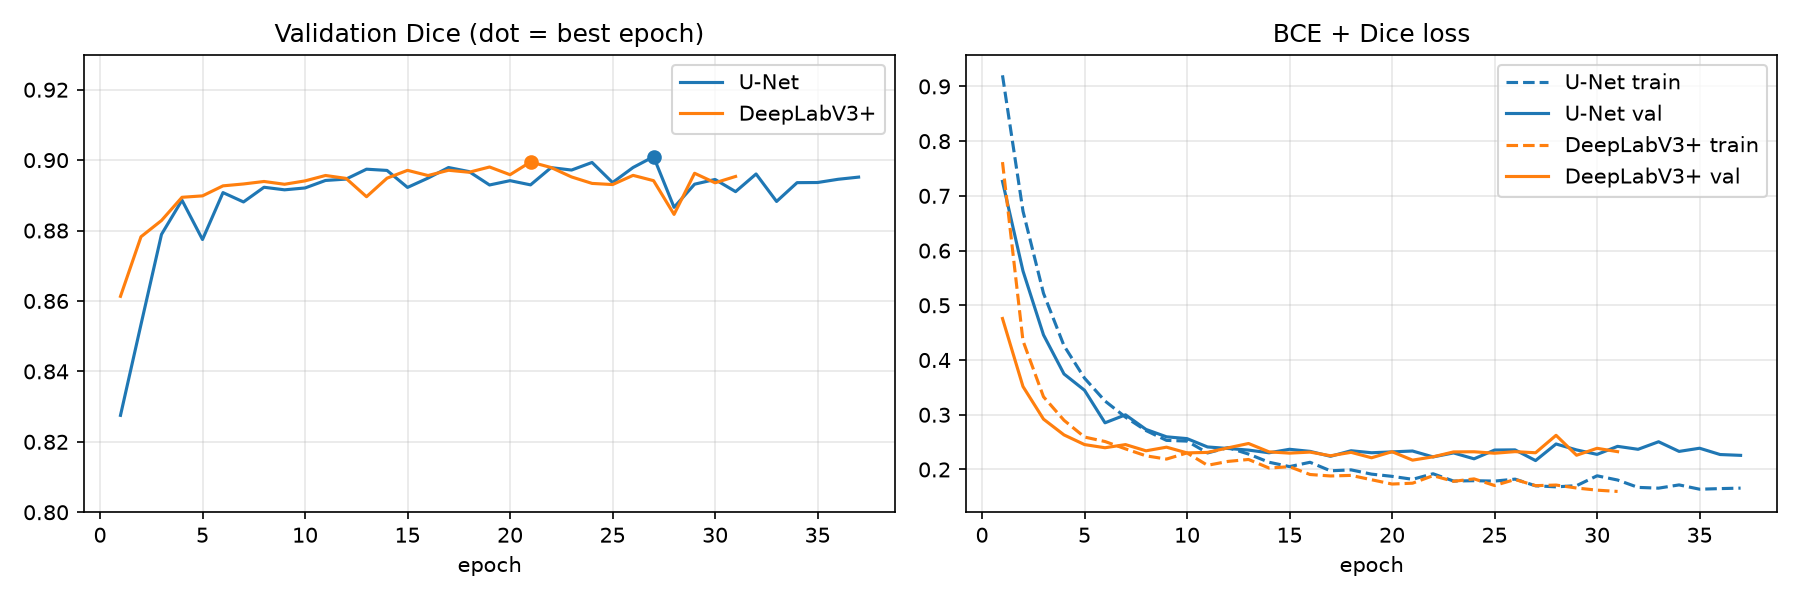
\includegraphics[width=0.9\linewidth]{figures/learning_curves_comparison.png}
\caption{Validation Dice (dot = best epoch) and training/validation loss of both models.}
\label{fig:curves}
\end{figure}

\begin{table}[htbp]
\centering
\begin{tabular}{lccc|lccc}
\toprule
\textbf{Lesion area} & $n$ & \textbf{U-Net} & \textbf{DLV3+} & \textbf{Diagnosis} & $n$ & \textbf{U-Net} & \textbf{DLV3+} \\
\midrule
$<5\%$ & 90 & 0.876 & 0.868 & Nevus & 263 & 0.917 & 0.912 \\
5--20\% & 140 & 0.895 & 0.900 & Melanoma (all) & 88 & 0.886 & 0.884 \\
20--50\% & 107 & 0.913 & 0.904 & Seborrheic keratosis & 38 & 0.828 & 0.851 \\
$>50\%$ & 52 & 0.935 & 0.943 & & & & \\
\bottomrule
\end{tabular}
\caption{Mean Dice by lesion size (share of the image) and by diagnosis.}
\end{table}

\textbf{Breakdown.} As expected, DeepLabV3+ is better on the largest lesions ($+0.008$) and worse
on the smallest ones ($-0.008$), where its coarser output and single skip connection matter most;
the image with the largest loss is a small nevus (1.8\% of the image) whose Dice falls from 0.83
to 0.29. It gains most on seborrheic keratoses ($+0.023$, only 38 images), the hardest class for
the baseline. All other differences are below 0.01.

\textbf{Speed.} Although DeepLabV3+ has fewer parameters, it is slower on the same machine: 94 vs.\
70\,s per training epoch and 17.0 vs.\ 10.5\,ms per image. The total amount of computation is almost
the same (7.9 vs.\ 7.8 GMAC per image), but the dilated last encoder stage works on $16\times16$
instead of $8\times8$ features, so the encoder costs 7.3 instead of 4.8 GMAC, and the dilated and
depthwise-separable convolutions probably run less efficiently on the MPS GPU. Its shorter total
training time (49.9 vs.\ 54.9 min) only comes from early stopping after fewer epochs and from
different hardware. The speed rows of Table~\ref{tab:results} were measured separately and are lower than the
per-epoch time of the full U-Net run on the M4 (about 89\,s with validation), because the fanless
MacBook Air slows down from heating during a long run: there the U-Net epoch time grew from 67\,s
to about 100\,s.

\textbf{Training curves} (Figure~\ref{fig:curves}). DeepLabV3+ starts higher (validation Dice 0.861
vs.\ 0.828 after the first epoch) and reaches its best Dice earlier (epoch 21 vs.\ 27), so early
stopping ends its training 6 epochs sooner. After about 10 epochs both models plateau at
0.89--0.90 with almost the same validation loss (best 0.217 vs.\ 0.216), and both show the same mild
overfitting.

\section{Next Steps}

\begin{itemize}[noitemsep]
\item Repeat both models with 3 random seeds to see whether the small differences are stable.
\item Boundary analysis: error near the lesion border and visual comparison of the images where
the two models disagree most (low contrast, bubbles and plates, small lesions).
\item Final evaluation of both models on the official 1,000-image test set.
\end{itemize}

\end{document}